% !TEX TS-program = xelatex
% !TEX encoding = UTF-8
% !Mode:: "TeX:UTF-8"

\documentclass[onecolumn,oneside]{SUSTechHomework}

\usepackage{float}

\author{胡玉斌}
\sid{11712121}

\title{Lab 9}
\coursecode{CS315}
\coursename{Computer Security}

\begin{document}
  \maketitle

  You need to submit a detailed lab report to describe what you have done and what you have observed. Please provide details using screen shots and code snippets. You also need to provide explanation to the observations that are interesting or surprising.

  \section*{Task 1}

  Report your results in the lab report and explain how you are able to achieve that.

    \begin{figure}[H]
      \centering
      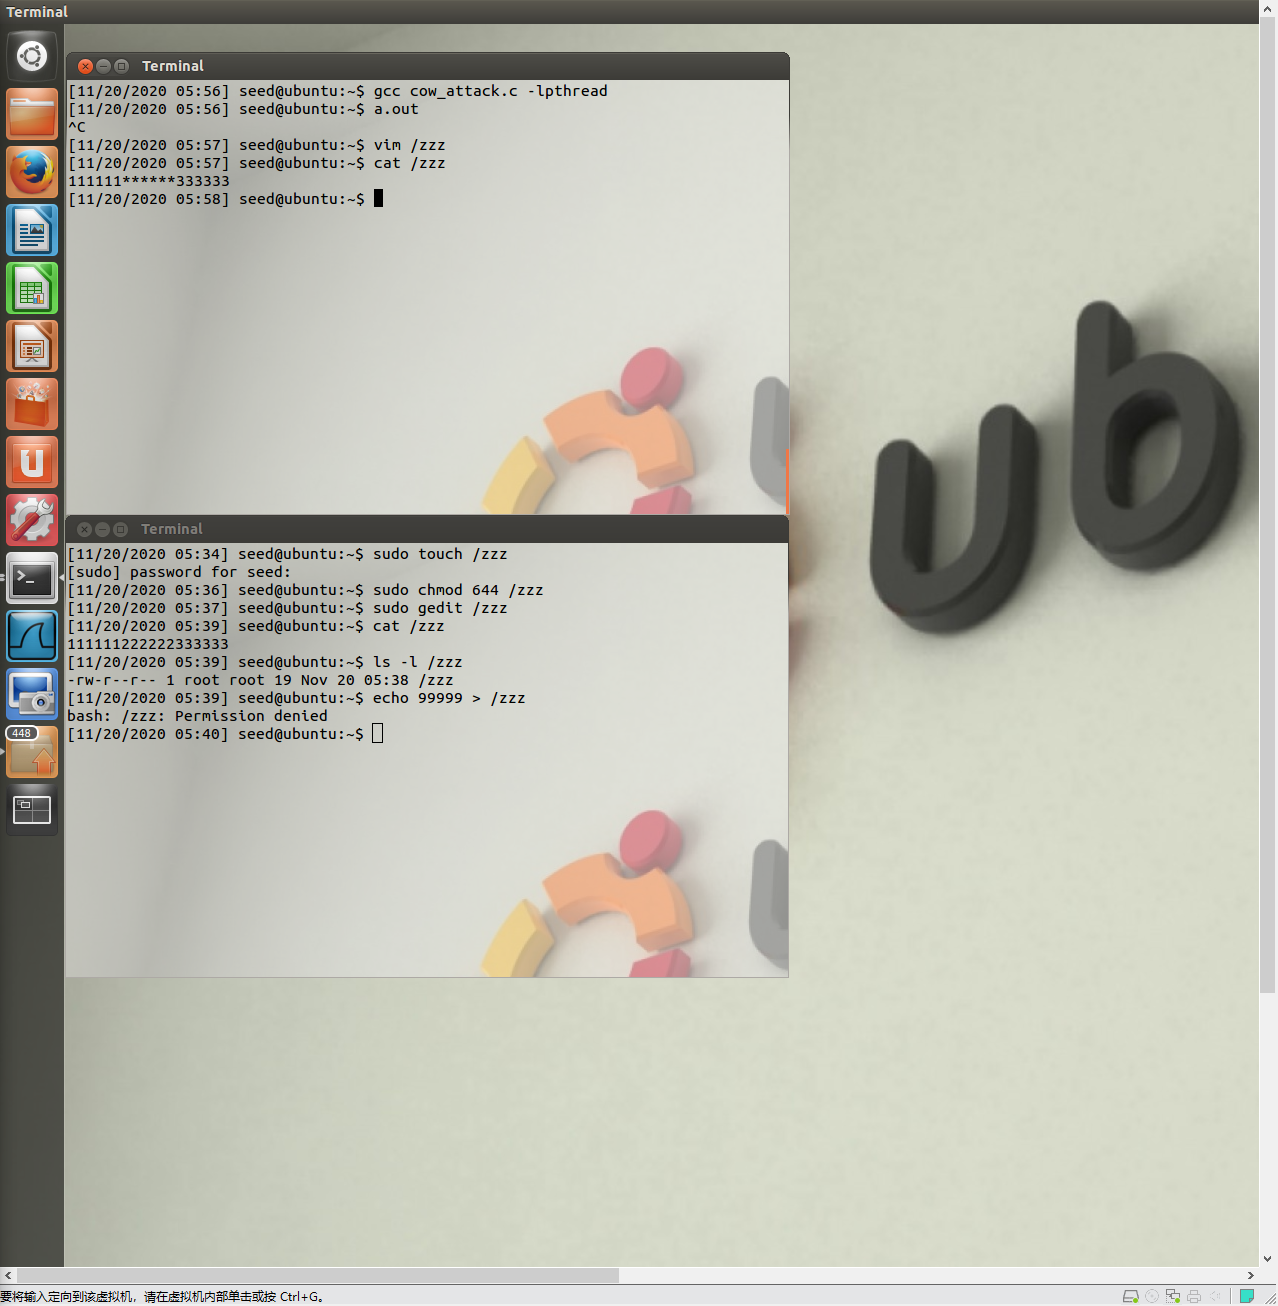
\includegraphics[width=0.85\textwidth]{img/pic1.png}
      \caption{read-only file}
    \end{figure}

    For Copy-On-Write, three important steps are performed:
    \begin{itemize}
      \item (A) Make a copy of the mapped memory
      \item (B) Update the page table, so the virtual memory points to newly created physical memory
      \item (C) Write to the memory.
    \end{itemize}
    The above steps are not atomic in nature: they can be interrupted by other threads which creates a potential race condition leading to Dirty Cow vulnerability.

    So when we execute \texttt{a.out}, we should press \texttt{Ctrl-C} after a few seconds and the attack succeeds.

  \section*{Task 2}

  We modify the code in \texttt{cow\_attack.c} as shown in Figure \ref{fig:code}, then do the similar operaion as in Task 1, then the attack succeeds.

    \begin{figure}[H]
      \centering
      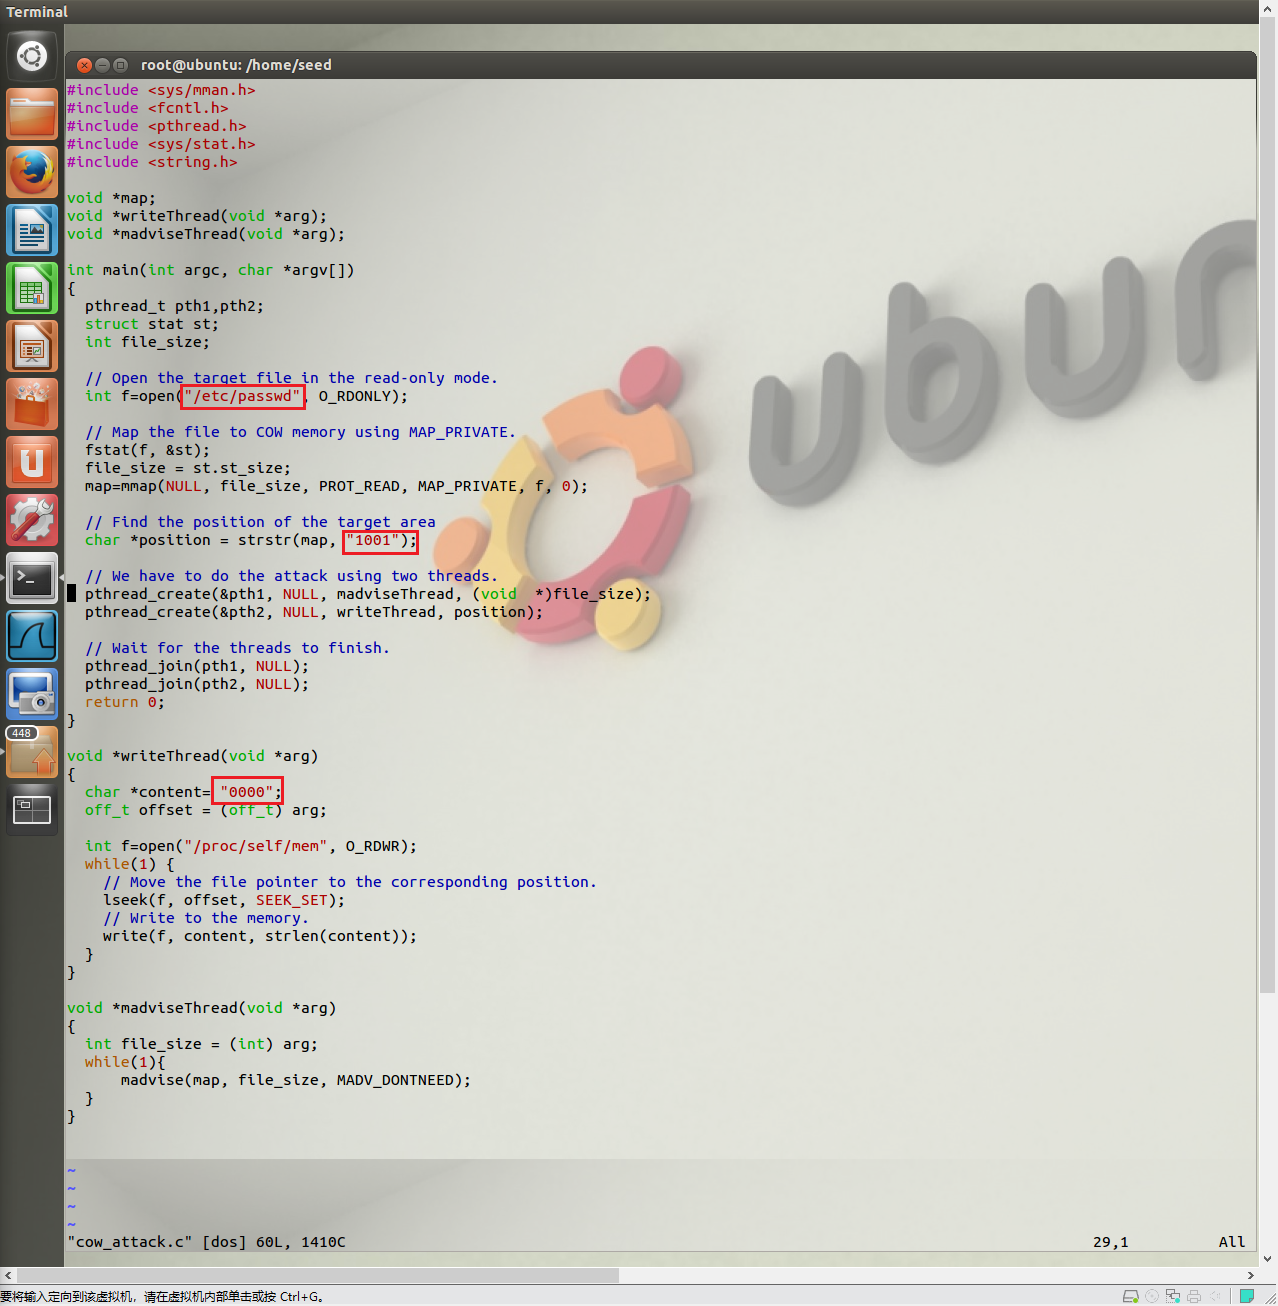
\includegraphics[width=0.85\textwidth]{img/pic3.png}
      \caption{code}
      \label{fig:code}
    \end{figure}

    \begin{figure}[H]
      \centering
      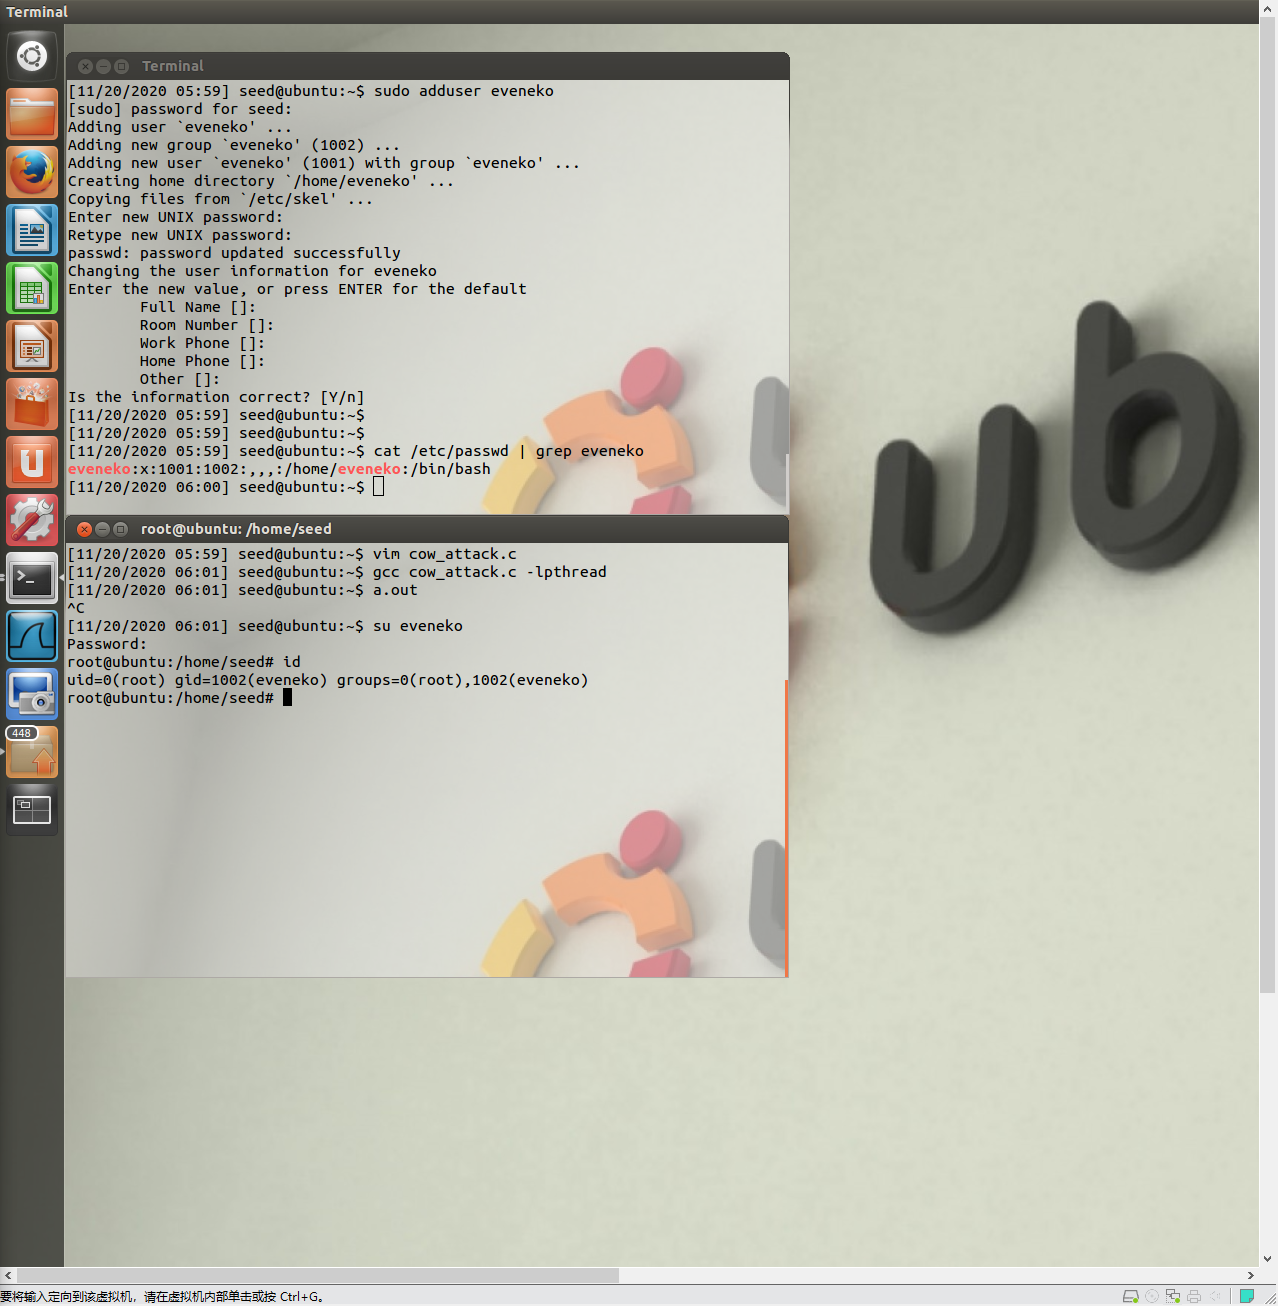
\includegraphics[width=0.85\textwidth]{img/pic2.png}
      \caption{root}
    \end{figure}


\end{document}
